\chapter{Génie génétique et biotechnologies}\label{ch:b3:genetic-engineering}

Jusqu'en 1982, tout diabétique du monde était maintenu en vie par de
l'insuline extraite du pancréas de porcs et de bovins --- quelque huit
mille kilogrammes de glandes pour un kilogramme d'hormone --- et une
fraction des patients réagissait contre la protéine étrangère. Cette
année-là, le premier médicament produit par un organisme génétiquement
modifié arrivait sur le marché~: de l'insuline humaine, synthétisée par
\emph{Escherichia coli} portant le gène humain sur un \omterm{def:b3:genetic-engineering:tools}{plasmide}. Les
outils qui l'avaient rendue possible avaient été rassemblés au cours de
la décennie précédente --- des enzymes qui coupent l'ADN à des
séquences choisies, des enzymes qui recollent les morceaux, des
\omterm{def:b3:genetic-engineering:tools}{plasmides} qui les emportent dans une cellule et les y recopient --- et
les décennies suivantes y ont ajouté la \omterm{def:b3:genetic-engineering:pcr}{réaction de polymérisation en
chaîne}, l'injection de gènes dans des embryons et, depuis 2012, un
système immunitaire bactérien transformé en ciseaux programmables
capables de réécrire une lettre d'un génome dans une cellule vivante.
Ce chapitre traite de ces outils, de l'arithmétique qui gouverne leur
emploi, et de ce qu'on a bâti avec eux, d'une souris luminescente à la
guérison de la drépanocytose.

\section{Couper, recoller et recopier l'ADN}

\begin{definition}[Enzymes de restriction, ligase et vecteurs]\label{def:b3:genetic-engineering:tools}
\index{enzyme de restriction}\index{extrémité cohésive}\index{ADN ligase}\index{vecteur}\index{plasmide}\index{marqueur de sélection}
Une \emph{enzyme de restriction} de type~II est une endonucléase
bactérienne qui coupe l'ADN double brin à une séquence précise de
\numrange{4}{8} paires de bases, le plus souvent palindromique~: EcoRI
coupe G$^{\downarrow}$AATTC, laissant des extrémités simple brin
sortantes de quatre bases (des \emph{extrémités cohésives})
complémentaires de toute autre extrémité EcoRI~; d'autres enzymes
laissent des \emph{extrémités franches}. L'\emph{ADN ligase} scelle
deux fragments dont les extrémités s'ajustent. Un \emph{vecteur} est
une molécule d'ADN qui se réplique dans un hôte et peut porter un
fragment inséré~: un \emph{plasmide} de quelques kilobases muni d'une
origine de réplication, d'un \emph{marqueur de sélection} (un gène de
résistance à un antibiotique, de sorte que seules les cellules ayant
capté le plasmide poussent sur l'antibiotique) et d'un groupe de sites
de restriction uniques pour l'insert~; le bactériophage $\lambda$, les
cosmides, et les chromosomes artificiels bactériens ou de levure pour
des inserts de \qtyrange{20}{1000}{kb}. L'ADN entre dans une bactérie
par \emph{transformation}, après un choc chimique ou électrique qui
rend la membrane transitoirement perméable, avec une efficacité de
$10^{6}$ à $10^{9}$ transformants par microgramme de plasmide. Une
molécule \emph{recombinante} est une molécule qui réunit de l'ADN de
deux provenances.
\end{definition}

\begin{proof}[Faits expérimentaux]
Cohen, Chang, Boyer et Helling (1973) ont coupé par EcoRI le \omterm{def:b3:genetic-engineering:tools}{plasmide}
pSC101 et un second \omterm{def:b3:genetic-engineering:tools}{plasmide} portant un autre gène de résistance,
mélangé et ligaturé les fragments, transformé \emph{E.~coli} et obtenu
des colonies résistantes aux deux antibiotiques, porteuses d'un unique
\omterm{def:b3:genetic-engineering:tools}{plasmide} fait des deux --- le premier ADN recombinant à se répliquer
dans une cellule. L'année suivante ils ont inséré dans pSC101 des gènes
d'ARN ribosomique de crapaud et montré que cet ADN d'amphibien était
répliqué, et transcrit, dans la bactérie~: les gènes franchissent la
frontière entre règnes sans changer, et une bactérie recopie l'ADN
qu'on lui donne, quel qu'il soit.
\end{proof}

\begin{omfigure}
\begin{tikzpicture}[every node/.style={font=\scriptsize}, >=stealth]
  % plasmid circle
  \draw[very thick, omDef] (0,0) circle (1.8);
  % ori
  \draw[very thick, omMeth!70!black] (0,0) ++(60:1.8) arc[start angle=60, end angle=100, radius=1.8]; \node[above right] at (80:1.95) {origine de réplication};
  % ampR
  \draw[very thick, omProp] (0,0) ++(160:1.8) arc[start angle=160, end angle=250, radius=1.8]; \node[left, align=right] at (205:2.0) {gène de\\résistance\\marqueur};
  % MCS with insert
  \draw[very thick, omThm] (0,0) ++(-40:1.8) arc[start angle=-40, end angle=10, radius=1.8]; \node[right, align=left] at (-15:2.0) {insert, ligaturé dans\\le site de restriction};
  \draw[omThm] (-40:1.7) -- (-40:1.95); \draw[omThm] (10:1.7) -- (10:1.95);
  \node at (0,0.25) {plasmide}; \node at (0,-0.15) {\qtyrange{3}{5}{kb}};
  % sticky ends detail
  \begin{scope}[xshift=5.7cm, yshift=0.8cm]
    \node[left, align=right] at (-0.2,0) {EcoRI};
    \node[font=\ttfamily\scriptsize, anchor=west] at (0,0.25) {5$'$-G\,\textcolor{omThm}{AATT}C-3$'$};
    \node[font=\ttfamily\scriptsize, anchor=west] at (0,-0.25) {3$'$-C\textcolor{omThm}{TTAA}\,G-5$'$};
    \draw[->, omThm, thick] (0.62,0.55) -- (0.62,0.3); \draw[->, omThm, thick] (1.62,-0.55) -- (1.62,-0.3);
    \node[anchor=west, align=left] at (2.9,0) {coupures décalées~:\\extrémités sortantes\\de quatre bases, cohésives};
  \end{scope}
  \begin{scope}[xshift=5.7cm, yshift=-1.3cm]
    \draw[very thick, omDef] (0,0.15) -- (1.2,0.15); \draw[very thick, omDef] (0,-0.15) -- (0.7,-0.15);
    \draw[very thick, omThm] (1.7,0.15) -- (3.0,0.15); \draw[very thick, omThm] (1.2,-0.15) -- (3.0,-0.15);
    \node[above] at (1.45,0.2) {appariement}; \node[below, align=center] at (1.5,-0.25) {deux bouts EcoRI s'apparient~;\\la ligase scelle le squelette};
  \end{scope}
\end{tikzpicture}

{\small Un \omterm{def:b3:genetic-engineering:tools}{vecteur} de clonage et sa chimie. Le \omterm{def:b3:genetic-engineering:tools}{plasmide} porte une
origine, un \omterm{def:b3:genetic-engineering:tools}{marqueur de sélection} et un site de restriction unique dans
lequel on ligature un fragment coupé par la même enzyme~; les
\omterm{def:b3:genetic-engineering:tools}{extrémités cohésives} rendent compatibles deux fragments quelconques
coupés par la même enzyme.}
\end{omfigure}

\begin{method}[Cloner un gène]\label{met:b3:genetic-engineering:cloning}
\index{clonage}\index{banque}\index{criblage}
(1) Se procurer l'insert~: couper l'ADN génomique par une \omterm{def:b3:genetic-engineering:tools}{enzyme de
restriction}, ou recopier un ARN messager en ADN complémentaire (ADNc,
dépourvu d'introns et donc exprimable dans une bactérie), ou amplifier
le gène par PCR avec des \omterm{def:b3:genetic-engineering:pcr}{amorces} portant des sites de restriction.
(2) Couper le \omterm{def:b3:genetic-engineering:tools}{vecteur} et l'insert par la ou les mêmes enzymes --- deux
enzymes différentes imposent l'orientation de l'insert --- et
ligaturer. (3) Transformer des bactéries et les étaler sur
l'antibiotique~: seules les cellules munies d'un \omterm{def:b3:genetic-engineering:tools}{plasmide} poussent.
(4) Distinguer les \omterm{def:b3:genetic-engineering:tools}{plasmides} porteurs d'un insert de ceux qui se sont
refermés sur eux-mêmes~: un gène marqueur interrompu par le site de
clonage (\emph{lacZ}~: les colonies blanches ont un insert, les bleues
non). (5) Cribler les colonies pour l'insert voulu~: par hybridation
avec une sonde marquée, par PCR, ou par digestion de restriction et
électrophorèse en gel. (6) Séquencer l'insert. Une \emph{banque} est
l'ensemble des clones issus d'un génome ou d'un transcriptome entier,
dans lequel on pêche n'importe quel gène par le même criblage.
\end{method}

\begin{omfigure}
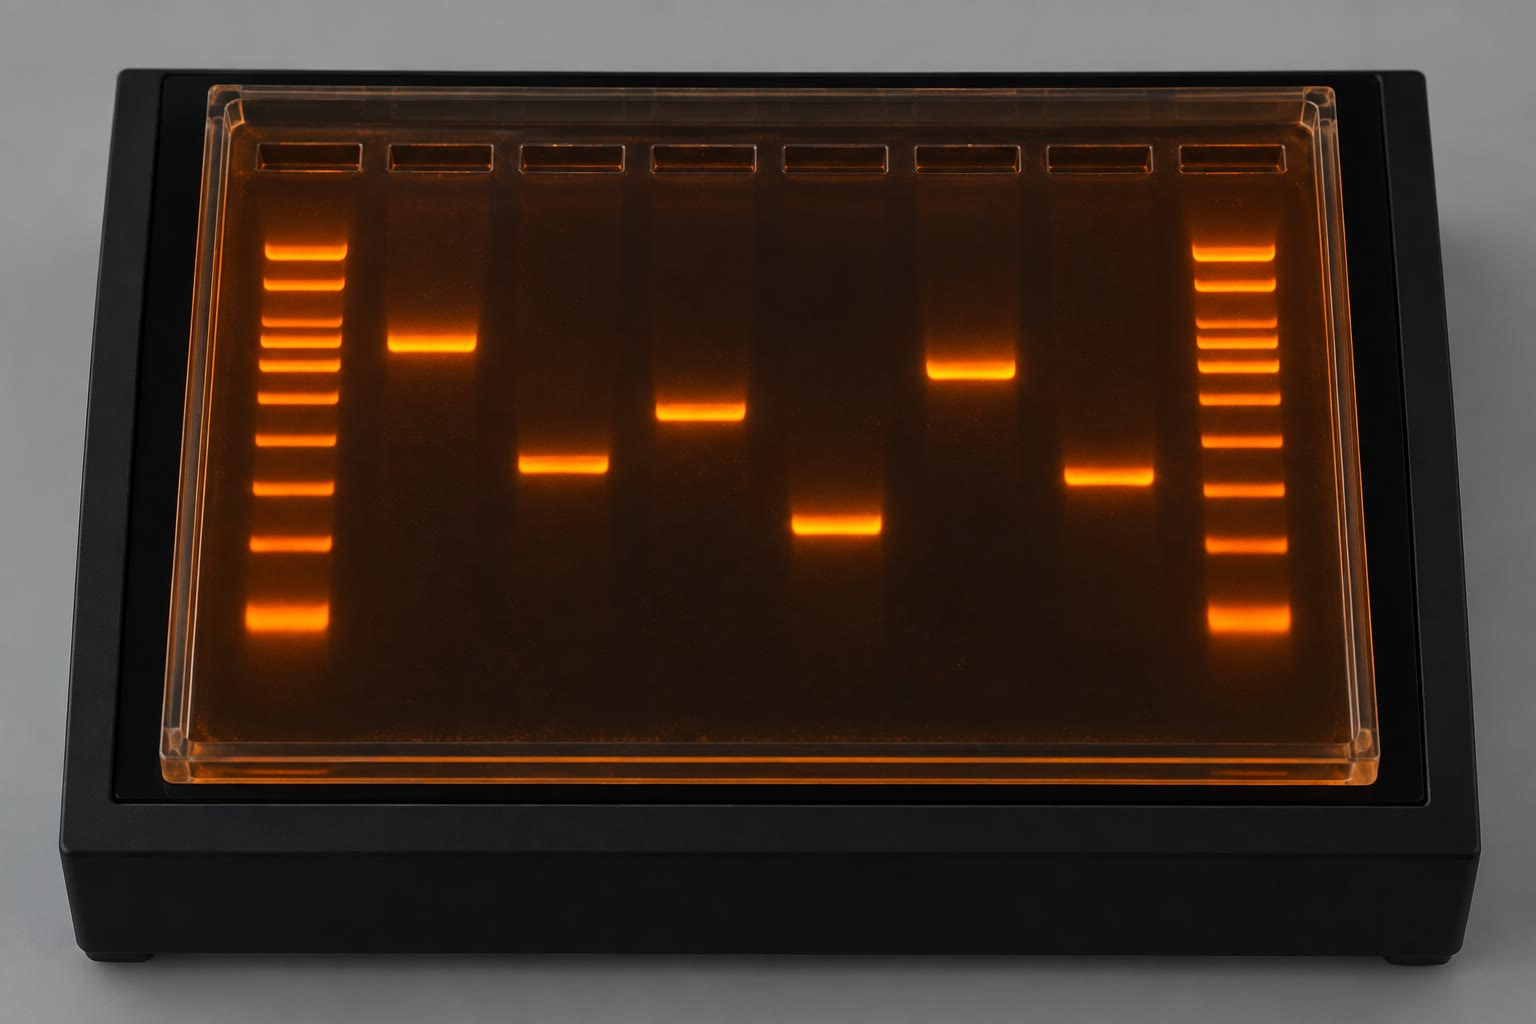
\includegraphics[width=0.56\linewidth]{images/book5/ai/b5-06-agarose-gel.jpg}

{\small Un gel d'agarose sous lumière ultraviolette~: les fragments
d'ADN migrent vers l'anode à une vitesse qui décroît avec leur
longueur, de sorte que chaque bande est une population de molécules
d'une même taille, comparée à l'échelle de tailles connues des pistes
extérieures.}
\end{omfigure}

\begin{definition}[La réaction de polymérisation en chaîne]\label{def:b3:genetic-engineering:pcr}
\index{réaction de polymérisation en chaîne}\index{amorce}\index{PCR quantitative}
La \emph{réaction de polymérisation en chaîne} (PCR) amplifie un
tronçon d'ADN choisi entre deux \emph{amorces} --- oligonucléotides de
synthèse d'une vingtaine de bases, complémentaires des deux brins aux
extrémités de la cible --- par des cycles de trois températures~:
\qty{95}{\celsius} pour séparer les brins,
\qtyrange{50}{65}{\celsius} pour que les amorces s'apparient,
\qty{72}{\celsius} pour qu'une polymérase thermostable (la Taq, tirée
de la bactérie des sources chaudes \emph{Thermus aquaticus}) les
prolonge. Chaque cycle double le nombre de copies du segment compris
entre les amorces, de sorte que trente cycles font d'une molécule
unique un milliard. La \emph{PCR après transcription inverse} recopie
d'abord l'ARN en ADN et mesure donc des transcrits ou des virus à
ARN~; la \emph{PCR quantitative} (qPCR) suit l'amplification en temps
réel grâce à un colorant fluorescent et lit la quantité de départ au
cycle où le signal franchit un seuil.
\end{definition}

\begin{theorem}[L'arithmétique de l'amplification]\label{thm:b3:genetic-engineering:pcr}
\index{cycle seuil}
Avec une efficacité $E$ par cycle ($E = 1$ pour un doublement parfait),
$N_{0}$ copies de départ deviennent
\[
N_{n} = N_{0}\,(1 + E)^{n}
\]
après $n$ cycles. Si la fluorescence franchit un seuil fixe lorsque le
nombre de copies atteint $N_{T}$, le \emph{\omterm{thm:b3:genetic-engineering:pcr}{cycle seuil}} vaut
\[
C_{T} = \frac{\log N_{T} - \log N_{0}}{\log(1 + E)},
\]
droite en $\log N_{0}$ de pente $-1/\log(1+E)$~: pour $E = 1$, chaque
augmentation d'un facteur dix de la quantité de départ abaisse $C_{T}$
de $\log_{2} 10 = 3.32$ cycles, et deux échantillons dont les \omterm{thm:b3:genetic-engineering:pcr}{cycles
seuils} diffèrent de $\Delta C_{T}$ diffèrent en copies de départ du
facteur $(1 + E)^{\Delta C_{T}}$.
\end{theorem}
\begin{proof}
Chaque cycle multiplie le nombre de copies par $1 + E$, donc $N_{n}$
est une suite géométrique. En posant $N_{n} = N_{T}$ et en résolvant en
$n$ on obtient $C_{T}$~; la pente est le coefficient de $\log N_{0}$.
Pour deux échantillons,
$C_{T,1} - C_{T,2} = (\log N_{0,2} - \log N_{0,1})/\log(1+E)$, d'où
$N_{0,2}/N_{0,1} = (1+E)^{\Delta C_{T}}$.
\end{proof}

\begin{example}[Lire une plaque de qPCR]\label{ex:b3:genetic-engineering:qpcr}
Un test d'ARN viral franchit le seuil au cycle $22$ chez un patient et
au cycle $32$ chez un autre~; avec $E \approx 1$ le premier porte $2^{10}
\approx 1000$ fois plus de virus. Un échantillon de dix copies franchit
le seuil vers le cycle $37$ quand celui-ci vaut $10^{12}$ copies
($\log_{2} 10^{11} =
36.5$)~; une course de $40$ cycles détecte donc quelques molécules ---
et une seule molécule contaminante d'un amplicon antérieur aussi, ce
qui explique que les laboratoires séparent les salles où l'on prépare
une PCR de celles où l'on manipule les produits.
\end{example}

\begin{omfigure}
\begin{tikzpicture}
\begin{axis}[
  width=0.7\linewidth, height=5.6cm,
  axis x line=bottom, axis y line=left,
  xmin=0, xmax=40, ymin=1, ymax=1e14, ymode=log,
  xlabel={cycle}, ylabel={copies},
  xlabel style={font=\small, at={(axis description cs:0.5,-0.12)}, anchor=north},
  ylabel style={font=\small},
  tick label style={font=\small}, xtick={0,10,20,30,40},
  clip=false,
]
\addplot[very thick, omDef, domain=0:40, samples=41] {1e7*2^x/(1+2^x/1e5)};
\addplot[very thick, omThm, domain=0:40, samples=41] {1e4*2^x/(1+2^x/1e8)};
\addplot[very thick, omMeth!70!black, domain=0:40, samples=41] {10*2^x/(1+2^x/1e11)};
\addplot[dashed, gray, domain=0:40, samples=2] {1e12};
\node[font=\scriptsize, gray, anchor=south west] at (axis cs:0.5,1.3e12) {seuil $N_{T}$};
\draw[gray] (axis cs:16.6,1) -- (axis cs:16.6,1e12); \draw[gray] (axis cs:26.6,1) -- (axis cs:26.6,1e12); \draw[gray] (axis cs:36.5,1) -- (axis cs:36.5,1e12);
\node[font=\scriptsize, anchor=south] at (axis cs:16.6,3e12) {$C_{T} = 16.6$}; \node[font=\scriptsize, anchor=south] at (axis cs:26.6,3e12) {$26.6$}; \node[font=\scriptsize, anchor=south] at (axis cs:36.5,3e12) {$36.5$};
\end{axis}
\end{tikzpicture}

{\small Courbes d'amplification pour $N_{0} = 10^{7}$ (bleu), $10^{4}$
(rouge) et $10$ copies (vert), $E = 1$, avec le plateau qu'imposent les
réactifs. Une différence d'un facteur mille sur $N_{0}$ décale le \omterm{thm:b3:genetic-engineering:pcr}{cycle
seuil} de $10$~; les plateaux se ressemblent tous, ce qui explique que
le produit final ne dise rien du départ.}
\end{omfigure}

\section{Fabriquer des protéines}

\begin{definition}[Systèmes d'expression]\label{def:b3:genetic-engineering:expression}
\index{vecteur d'expression}\index{protéine recombinante}\index{anticorps monoclonal}
Un \emph{\omterm{def:b3:genetic-engineering:tools}{vecteur} d'expression} place la séquence codante clonée sous un
promoteur fort et contrôlable de l'hôte (le promoteur \emph{lac} ou T7
chez \emph{E.~coli}, induit par un analogue de sucre), avec un site de
fixation du ribosome, un terminateur, et souvent une \emph{étiquette}
--- six histidines, une petite protéine --- fusionnée au produit pour
sa purification sur colonne. Les bactéries fabriquent des grammes par
litre d'une protéine simple (insuline, hormone de croissance, enzymes)
mais ne savent ni glycosyler ni replier les protéines complexes de
mammifère~; la levure ajoute des sucres qui lui sont propres~; les
cellules d'insecte et de mammifère (les cellules d'ovaire de hamster
chinois sont la norme industrielle) fabriquent des anticorps et des
facteurs de coagulation repliés et glycosylés comme chez l'homme. Un
\emph{anticorps monoclonal} est produit par un \emph{hybridome} --- un
lymphocyte~B producteur d'anticorps fusionné à une cellule de myélome
immortelle (Köhler et Milstein, 1975) --- ou, aujourd'hui, en clonant
les gènes de l'anticorps dans une lignée d'expression de mammifère, où
la charpente murine peut être remplacée par de la séquence humaine pour
éviter le rejet immunitaire (\cref{ch:b3:adaptive-immunity}).
\end{definition}

\begin{example}[L'insuline]\label{ex:b3:genetic-engineering:insulin}
L'insuline humaine est faite de deux chaînes, A (21 résidus) et B
(30), unies par des ponts disulfure et découpées dans la cellule
$\beta$ à partir d'un unique précurseur, la proinsuline. Le premier
procédé exprimait les deux chaînes séparément chez \emph{E.~coli},
chacune fusionnée à la $\beta$-galactosidase, les en détachait
chimiquement et les unissait in vitro~; les procédés ultérieurs
expriment la proinsuline et la clivent par les enzymes qu'emploie le
pancréas. Depuis 1996 la séquence elle-même est modifiée~: échanger ou
ajouter un résidu ou deux donne des analogues qui se dissocient plus
vite (pour un repas) ou précipitent au point d'injection et se libèrent
sur une journée. Une protéine qui coûtait huit tonnes de glandes par
kilogramme se fabrique aujourd'hui dans un fermenteur, identique à
l'humaine ou meilleure qu'elle.
\end{example}

\section{Organismes transgéniques}

\begin{definition}[Transgenèse et ciblage de gènes]\label{def:b3:genetic-engineering:transgenic}
\index{organisme transgénique}\index{microinjection}\index{knock-out}\index{cellule souche embryonnaire}\index{ciblage de gènes}
Un organisme \emph{transgénique} porte un gène introduit dans sa lignée
germinale, de sorte que toutes ses cellules l'ont et qu'il est hérité.
Chez la souris la voie classique est la \emph{microinjection} de l'ADN
dans un pronucléus d'un œuf fécondé (Gordon et Ruddle, 1980), qui
l'intègre en un site au hasard chez une fraction des embryons~;
Palmiter et Brinster (1982) ont obtenu des souris de taille double en
injectant le gène de l'hormone de croissance de rat derrière un
promoteur de métallothionéine. Le \emph{ciblage de gènes} remplace ou
interrompt plutôt un gène choisi~: une construction munie de longs bras
homologues de la cible est introduite dans des \emph{cellules souches
embryonnaires}, les rares cellules où la \omterm{def:b3:dna-repair:dsb}{recombinaison homologue} l'a
mise au bon endroit sont sélectionnées et injectées dans un
blastocyste, et la souris chimère qui en résulte transmet le gène
modifié (Capecchi, Smithies et Evans, années 1980). Un
\emph{knock-out} n'a plus le gène~; un \emph{knock-in} en porte une
version modifiée~; un allèle \emph{conditionnel}, encadré de sites
loxP, n'est supprimé que là et quand Cre est exprimée
(\cref{ch:b3:dna-repair}). Une dizaine de milliers de gènes de souris
ont été invalidés, et pour la plupart le phénotype a été le premier
indice de ce que fait le gène.
\end{definition}

\begin{omfigure}
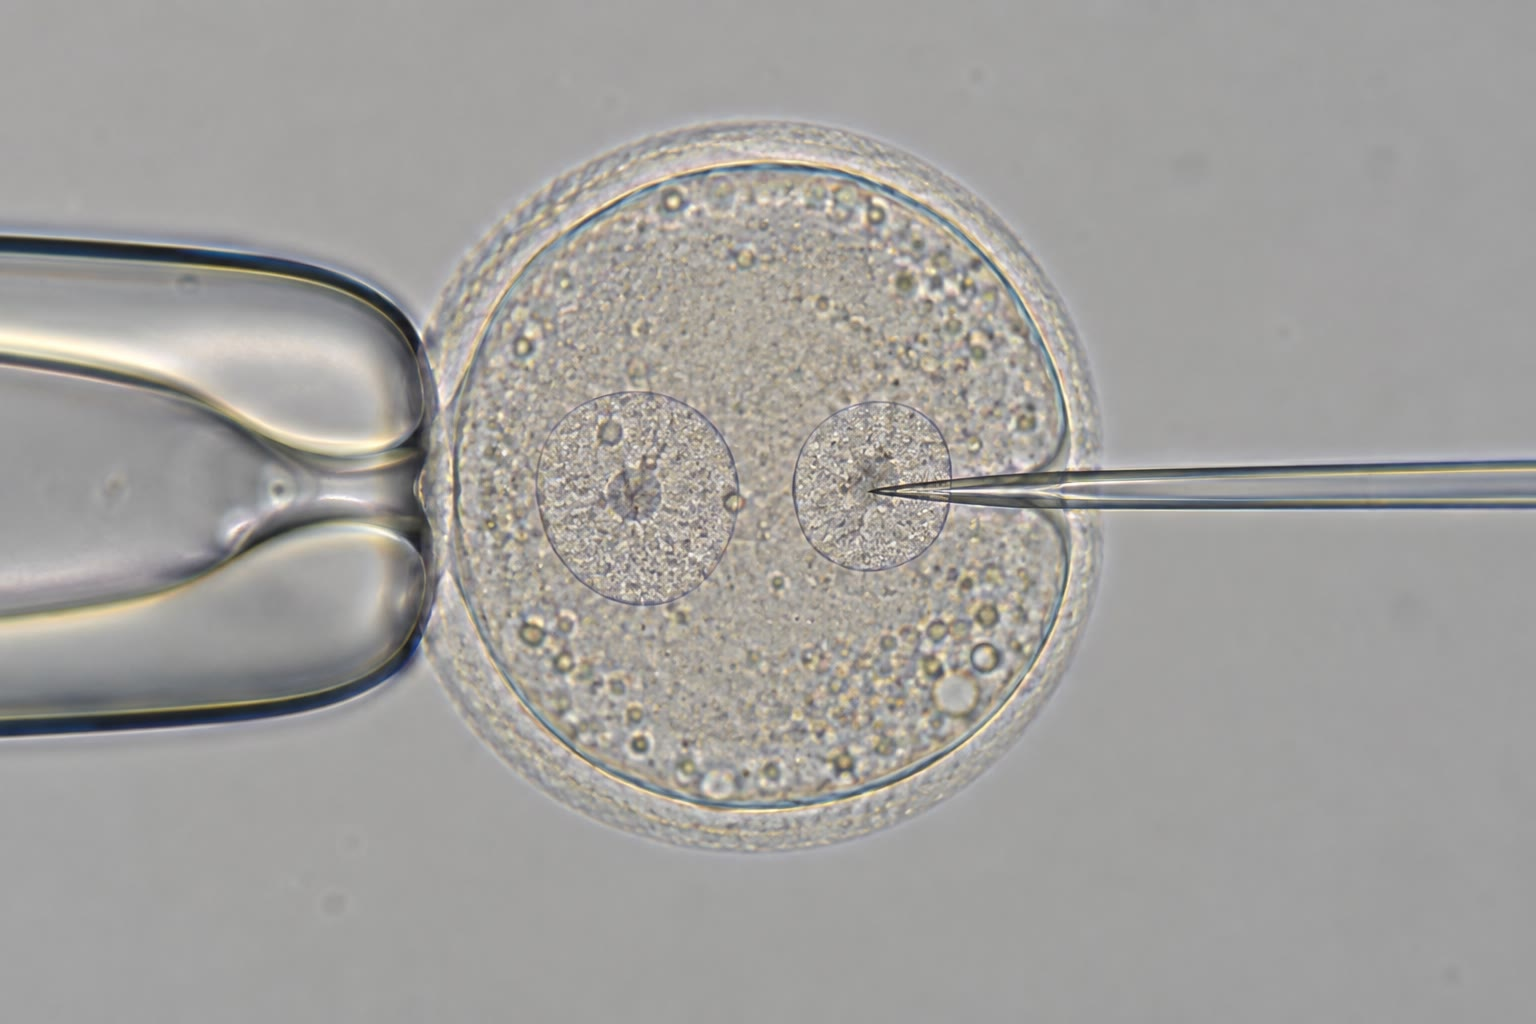
\includegraphics[width=0.46\linewidth]{images/book5/ai/b5-06-microinjection.jpg}\hspace{0.04\linewidth}
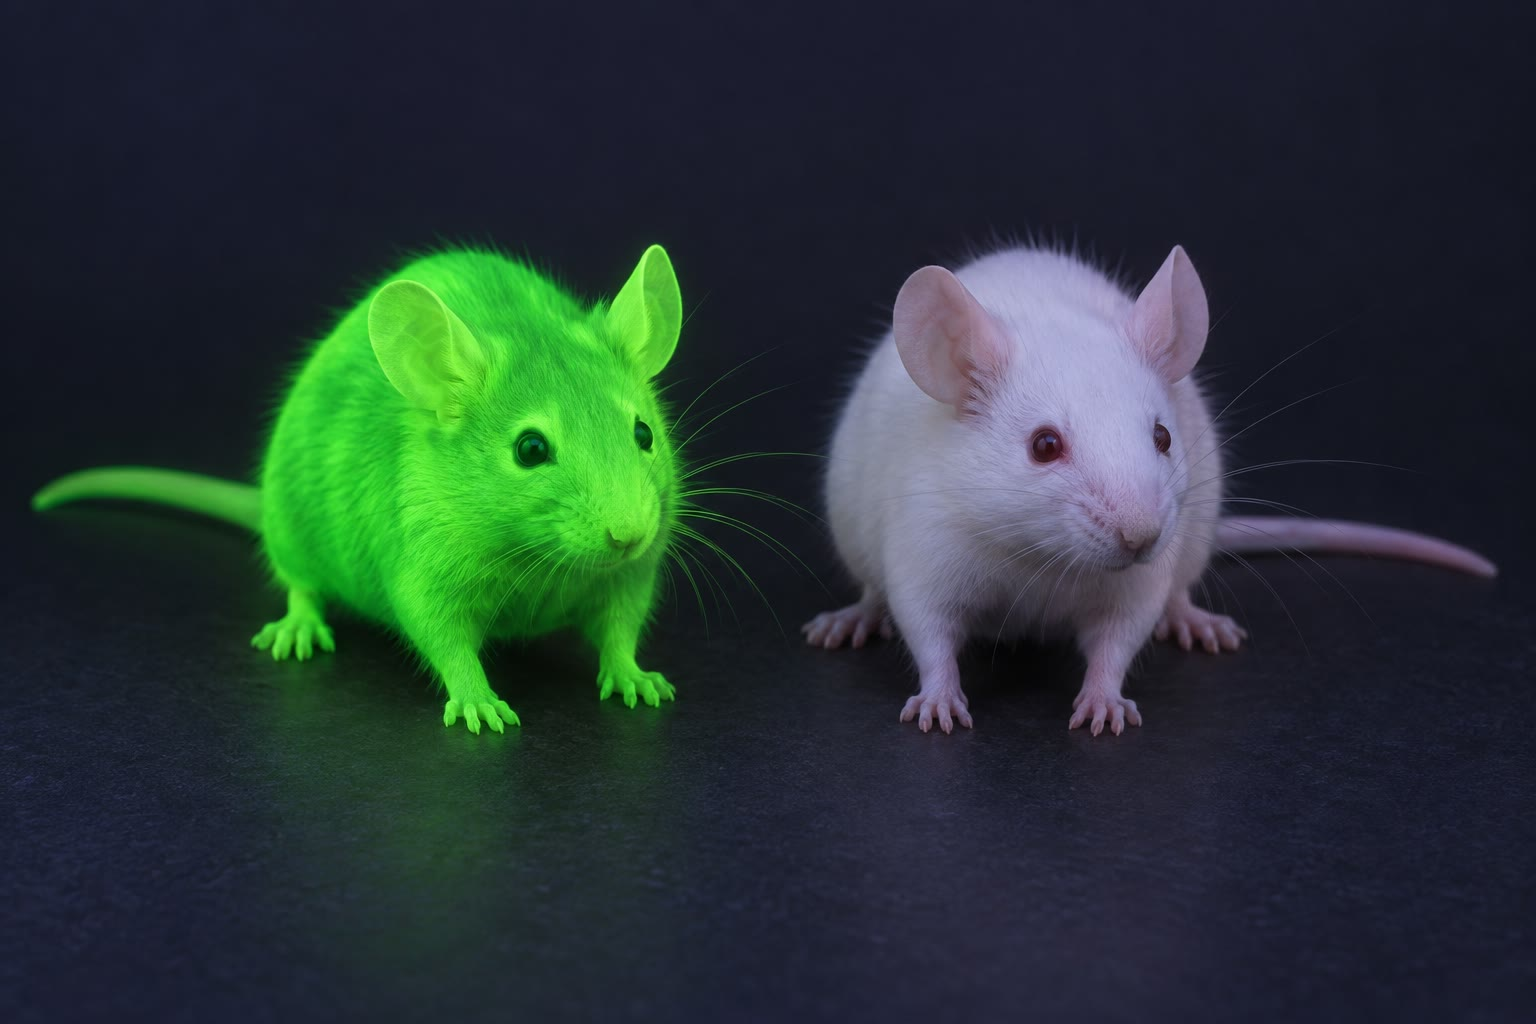
\includegraphics[width=0.46\linewidth]{images/book5/ai/b5-06-gfp-mouse.jpg}

{\small À gauche~: un œuf de souris fécondé, maintenu par aspiration
pendant qu'une aiguille de verre injecte de l'ADN dans un pronucléus. À
droite~: une souris \omterm{def:b3:genetic-engineering:transgenic}{transgénique} exprimant dans chaque cellule la
protéine fluorescente verte d'une méduse, à côté d'une sœur de portée
ordinaire, sous lumière ultraviolette.}
\end{omfigure}

\begin{definition}[Plantes transgéniques]\label{def:b3:genetic-engineering:plants}
\index{Agrobacterium}\index{ADN-T}\index{culture génétiquement modifiée}
Les plantes sont transformées par \emph{Agrobacterium tumefaciens},
bactérie du sol qui insère naturellement un segment de son \omterm{def:b3:genetic-engineering:tools}{plasmide}
inducteur de tumeur, l'\emph{ADN-T}, dans le génome d'une plante
blessée pour lui faire produire une galle qui la nourrit. Remplacer les
gènes propres de l'ADN-T par le gène de son choix, entre les séquences
de bordure que la bactérie reconnaît, fait du pathogène un \omterm{def:b3:genetic-engineering:tools}{vecteur}~;
les cellules transformées sont sélectionnées puis régénérées en plantes
entières, ce que sait faire toute cellule végétale. Les espèces que la
bactérie n'infecte pas (les céréales, longtemps) sont transformées en
tirant dans le tissu des particules d'or enrobées d'ADN. Les
\emph{cultures génétiquement modifiées} exploitées à grande échelle
portent un gène de toxine bactérienne (\emph{Bt}) contre les larves
d'insectes, ou une enzyme bactérienne conférant la tolérance à un
herbicide, ou les deux~; le \emph{riz doré} porte deux gènes de la voie
des caroténoïdes (une phytoène synthase végétale et une désaturase
bactérienne) de sorte que son albumen fabrique du $\beta$-carotène,
précurseur de la vitamine~A, dont la carence rend aveugle et tue
plusieurs centaines de milliers d'enfants par an.
\end{definition}

\begin{omfigure}
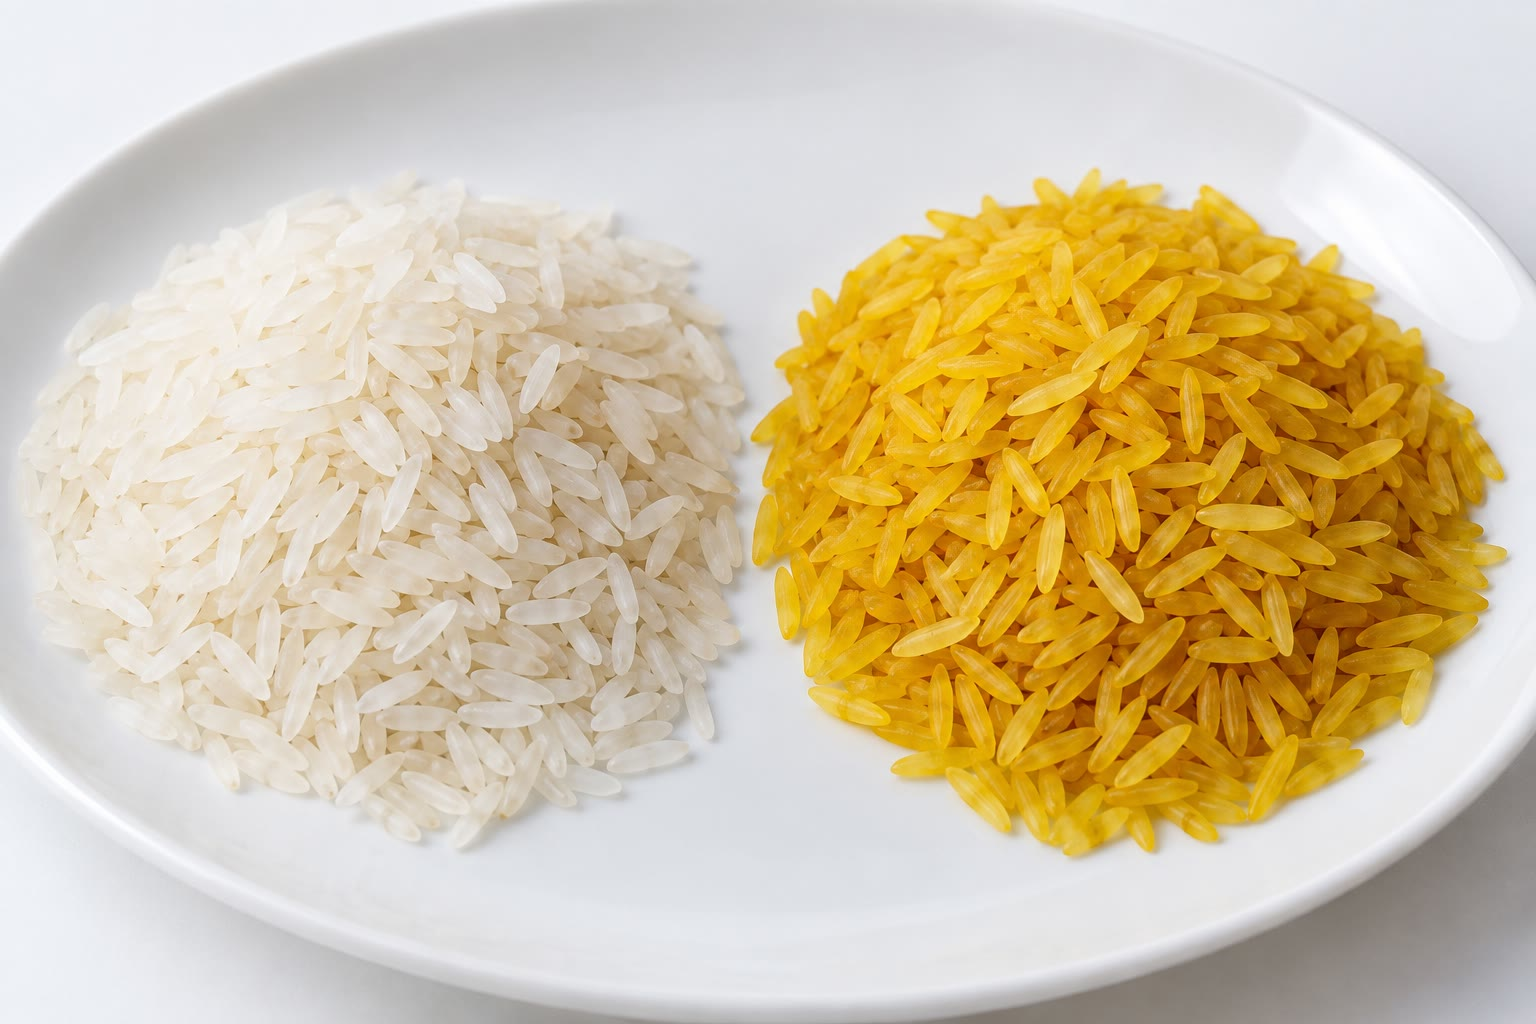
\includegraphics[width=0.46\linewidth]{images/book5/ai/b5-06-golden-rice.jpg}\hspace{0.04\linewidth}
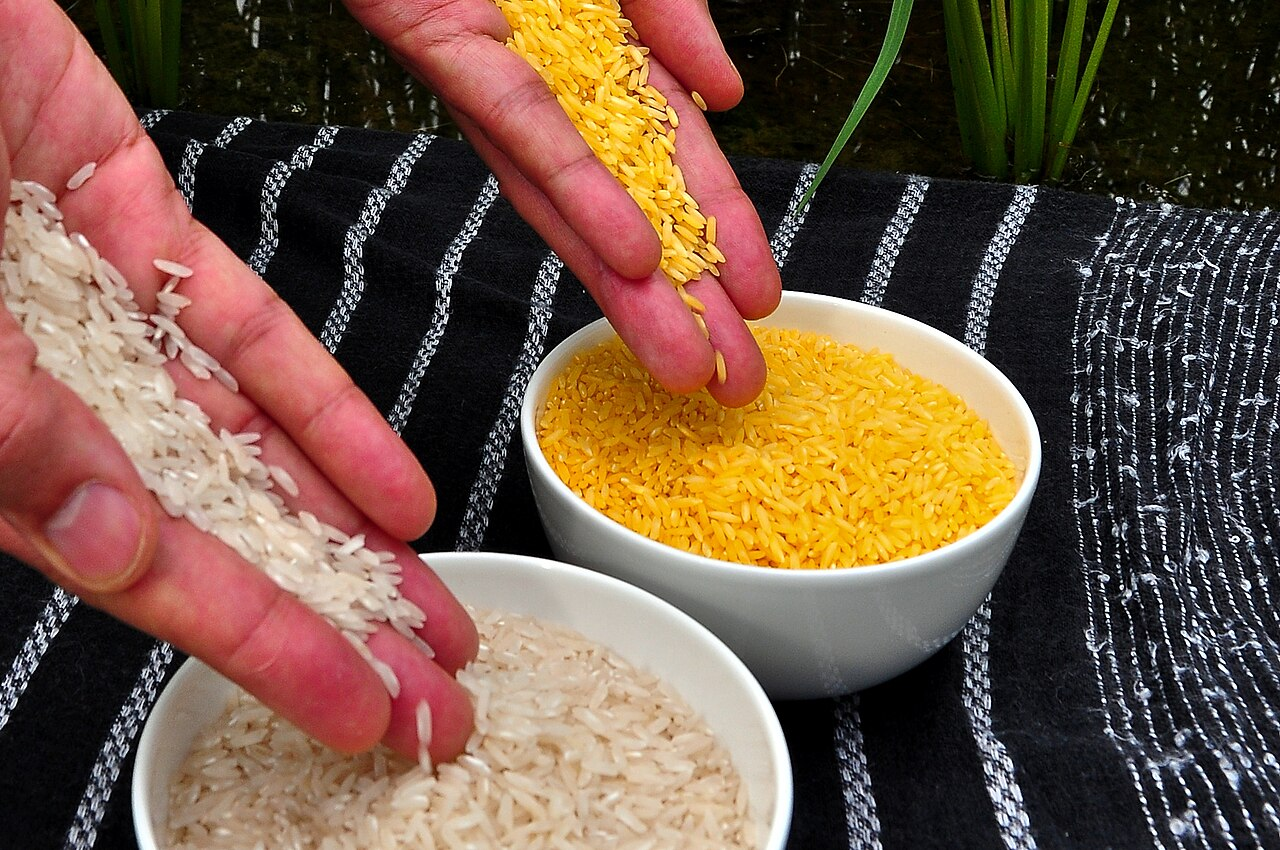
\includegraphics[width=0.46\linewidth]{images/book5/golden-rice-irri.jpg}

{\small Du riz ordinaire et du riz doré. Le grain jaune fabrique du
$\beta$-carotène dans son albumen grâce à deux gènes ajoutés de la voie
des caroténoïdes. À droite~: les deux riz comparés à l'Institut
international de recherche sur le riz (IRRI, CC~BY~2.0).}
\end{omfigure}

\begin{remark}[Le débat]\label{rem:b3:genetic-engineering:gmo}
Trente ans de culture sur des centaines de millions d'hectares, et
toutes les revues systématiques des académies scientifiques, n'ont
trouvé aux cultures \omterm{def:b3:genetic-engineering:transgenic}{transgéniques} autorisées aucun effet sanitaire qui
les distingue de leurs équivalents conventionnels~; le transgène est un
gène de plus parmi quarante mille, et la protéine qu'il fabrique est
testée comme l'est tout additif alimentaire. Les vraies questions sont
écologiques et économiques~: l'installation de résistances chez les
ravageurs et les adventices sous une sélection uniforme, le flux de
gènes vers les parents sauvages, la concentration du marché des
semences, et à qui profite l'affaire. Ce sont les questions que pose
toute technique agricole puissante, et les réponses dépendent du
caractère et du contexte, non de la méthode par laquelle le gène a été
déplacé.
\end{remark}

\section{Éditer les génomes}

\begin{definition}[CRISPR--Cas9]\label{def:b3:genetic-engineering:crispr}
\index{CRISPR}\index{Cas9}\index{ARN guide}\index{PAM}\index{édition du génome}
Les bactéries conservent dans un réseau de répétitions (\emph{CRISPR})
des fragments des génomes de phages qui ont infecté leurs ancêtres, les
transcrivent en courts ARN guides et s'en servent pour diriger une
nucléase sur tout ADN correspondant qui entre dans la cellule~: un
système immunitaire adaptatif doté d'une mémoire génétique. Chez
\emph{Streptococcus pyogenes} la nucléase est la protéine unique
\emph{Cas9}, qui fixe un ARN guide et un second petit ARN, cherche dans
l'ADN un \emph{motif adjacent au protospaceur} de trois bases (PAM,
5$'$-NGG), déroule l'ADN voisin et, si les vingt bases qui jouxtent le
PAM s'apparient au guide, coupe les deux brins à trois bases du PAM.
Jinek, Charpentier, Doudna et leurs collègues (2012) ont fusionné les
deux ARN en un unique \emph{ARN guide simple} et montré que Cas9, munie
d'un guide de séquence quelconque, coupe l'ADN à cette séquence dans un
tube à essai~; en un an on avait montré que le couple fonctionne dans
des cellules humaines, murines, de poisson-zèbre, de plante et de
levure. L'\emph{édition du génome} est ce que la cellule fait de la
coupure~: la jonction d'extrémités laisse une petite insertion ou
délétion qui interrompt le gène (une invalidation en une étape, chez
n'importe quel organisme, en quelques semaines), et la \omterm{def:b3:dna-repair:dsb}{recombinaison
homologue} avec une matrice fournie y écrit une séquence choisie.
\end{definition}

\begin{omfigure}
\begin{tikzpicture}[every node/.style={font=\scriptsize}, >=stealth]
  % Cas9 outline (drawn first so labels stay on top)
  \draw[thick, omExo, fill=omExo!15] (5.9,1.1) ellipse (2.6 and 1.6);
  \node[omExo!60!black] at (7.7,2.3) {Cas9};
  % target DNA
  \draw[very thick, omDef] (0,0.3) -- (11,0.3); \draw[very thick, omDef] (0,-0.1) -- (11,-0.1);
  % PAM
  \fill[omProp!60] (7.2,-0.2) rectangle (7.9,0.4); \node[below] at (7.55,-0.25) {PAM (NGG)};
  % protospacer
  \draw[omThm, very thick] (4.2,0.5) -- (7.15,0.5); \node[above] at (5.7,0.55) {cible de 20 bases, appariée au guide};
  % guide RNA
  \draw[very thick, omMeth!70!black] (4.2,0.3) .. controls (4.2,1.6) and (5.0,1.9) .. (5.4,1.9) -- (6.6,1.9) .. controls (7.0,1.9) and (7.2,2.5) .. (6.8,2.8) .. controls (6.3,3.1) and (5.8,2.7) .. (6.1,2.4);
  \node[left, omMeth!70!black, align=right] at (3.2,2.2) {ARN guide simple~:\\20 bases au choix\\+ tige-boucle de fixation de Cas9};
  % cut
  \draw[omThm, very thick, ->] (6.25,-0.7) -- (6.25,0.35); \node[omThm, below] at (6.25,-0.7) {cassure double brin, à 3 bases du PAM};
  % outcomes
  \draw[->, thick] (2.0,-1.3) -- (2.0,-1.9); \node[below, align=center] at (2.0,-1.9) {jonction d'extrémités~:\\petite insertion ou délétion\\$\Rightarrow$ décalage du cadre, invalidation};
  \draw[->, thick] (10.0,-1.3) -- (10.0,-1.9); \node[below, align=center] at (10.0,-1.9) {recombinaison avec une\\matrice fournie\\$\Rightarrow$ changement précis};
\end{tikzpicture}

{\small \omterm{def:b3:genetic-engineering:crispr}{Cas9} et son guide. La protéine se fixe à un \omterm{def:b3:genetic-engineering:crispr}{PAM}, déroule l'ADN
qui le jouxte et coupe si les vingt bases s'apparient à l'\omterm{def:b3:genetic-engineering:crispr}{ARN guide}. La
cassure est réparée soit par jonction d'extrémités, qui interrompt le
gène, soit par recombinaison avec une matrice, qui le réécrit.}
\end{omfigure}

\begin{proposition}[Éditer sans cassure]\label{prop:b3:genetic-engineering:editors}
\index{éditeur de bases}\index{éditeur prime}\index{site hors cible}
Couper les deux brins est l'édition la plus grossière~: l'issue de la
jonction d'extrémités est aléatoire, et une cassure ailleurs --- à un
\emph{\omterm{prop:b3:genetic-engineering:editors}{site hors cible}} qui diffère du guide en quelques positions, ce
que \omterm{def:b3:genetic-engineering:crispr}{Cas9} tolère --- est une mutation dont personne n'a voulu. Une \omterm{def:b3:genetic-engineering:crispr}{Cas9}
dont un domaine nucléase est inactivé n'entaille qu'un brin~; les deux
inactivés, elle se contente de se fixer et peut porter d'autres enzymes
jusqu'à une séquence. Les \emph{\omterm{prop:b3:genetic-engineering:editors}{éditeurs de bases}} fusionnent une \omterm{def:b3:genetic-engineering:crispr}{Cas9}
entaillante à une désaminase qui convertit C en U (lu T) ou A en I (lu
G) dans le brin déroulé, changeant une base sans cassure ni matrice~;
les \emph{\omterm{prop:b3:genetic-engineering:editors}{éditeurs prime}} portent une transcriptase inverse et un guide
prolongé par la séquence désirée, et recopient cette séquence dans le
brin entaillé, ce qui autorise toute substitution ainsi que de petites
insertions ou délétions. L'activité hors cible se réduit par des
variantes de \omterm{def:b3:genetic-engineering:crispr}{Cas9} de haute fidélité, en apportant l'enzyme brièvement
sous forme de protéine plutôt que de gène, et en choisissant des guides
dont les plus proches parents génomiques diffèrent en plusieurs
positions~; elle se mesure en séquençant les sites prédits et par des
méthodes non biaisées qui attrapent toute cassure du génome.
\end{proposition}

\begin{example}[Une guérison]\label{ex:b3:genetic-engineering:sickle}
La drépanocytose est un changement d'une seule base de la
$\beta$-globine. L'hémoglobine fœtale, faite de $\gamma$-globine, y
suppléerait, mais les gènes $\gamma$ sont éteints après la naissance
par le répresseur BCL11A. La première thérapie \omterm{def:b3:genetic-engineering:crispr}{CRISPR} autorisée (2023)
prélève les cellules souches sanguines du patient, coupe par \omterm{def:b3:genetic-engineering:crispr}{Cas9}
l'amplificateur érythroïde de \emph{BCL11A} de sorte que la jonction
d'extrémités le désactive dans la plupart des cellules, et rend les
cellules après que la moelle du patient a été vidée~: les globules
rouges qu'elles produisent sont riches en hémoglobine fœtale, ne
falciforment pas, et les crises cessent. L'édition est somatique --- la
lignée germinale n'est pas touchée et le changement ne s'hérite pas ---
et elle emploie l'issue «~grossière~», l'interruption, là où
l'interruption est ce que l'on veut.
\end{example}

\begin{theorem}[Propagation supra-mendélienne d'un forçage génétique]\label{thm:b3:genetic-engineering:drive}
\index{forçage génétique}
Un \emph{\omterm{thm:b3:genetic-engineering:drive}{forçage génétique}} est une construction codant \omterm{def:b3:genetic-engineering:crispr}{Cas9} et un
guide qui coupe l'allèle sauvage à son propre locus chez un
hétérozygote~; la réparation par recombinaison recopie le forçage dans
le chromosome coupé, de sorte qu'une fraction $c$ des gamètes de
l'hétérozygote porte le forçage au lieu de la moitié mendélienne. Si le
forçage a la fréquence $p$ dans une grande population à panmixie et
n'entraîne aucun coût de valeur sélective, sa fréquence à la génération
suivante vaut
\[
p' = p + c\,p\,(1 - p),
\]
de sorte qu'il se propage depuis la rareté à une vitesse
proportionnelle à $c$, et atteint la moitié de la population en
environ $\ln(1/p_{0})/\ln(1 + c)$ générations à partir d'une fréquence
initiale $p_{0}$.
\end{theorem}
\begin{proof}
La panmixie donne des homozygotes pour le forçage à la fréquence
$p^{2}$, des hétérozygotes à $2p(1-p)$, des homozygotes sauvages à
$(1-p)^{2}$. Les homozygotes transmettent le forçage à tous leurs
gamètes, les hétérozygotes à une fraction $(1 + c)/2$ (la moitié par
Mendel, plus $c$ fois la moitié sauvage convertie), les sauvages à
aucun. D'où $p' = p^{2} + 2p(1-p)(1+c)/2
= p^{2} + p(1-p) + c\,p(1-p) = p + c\,p(1-p)$. Pour $p$ petit cela vaut
$p' \approx (1+c)p$, une croissance géométrique de raison $1 + c$, qui
atteint $1/2$ depuis $p_{0}$ après environ
$\ln(1/2p_{0})/\ln(1+c)$ générations~; le terme logistique ne la
ralentit qu'à la toute fin.
\end{proof}

\begin{omfigure}
\begin{tikzpicture}
\begin{axis}[
  width=0.7\linewidth, height=5.6cm,
  axis x line=bottom, axis y line=left,
  xmin=0, xmax=20, ymin=0, ymax=1.05,
  xlabel={génération}, ylabel={fréquence du forçage $p$},
  xlabel style={font=\small, at={(axis description cs:0.5,-0.12)}, anchor=north},
  ylabel style={font=\small},
  tick label style={font=\small}, xtick={0,5,10,15,20}, ytick={0,0.5,1},
  clip=false,
]
\addplot[very thick, omThm, mark=*, mark size=1.2pt] coordinates {(0,0.01) (1,0.0189) (2,0.0356) (3,0.0665) (4,0.1224) (5,0.2191) (6,0.3731) (7,0.5836) (8,0.8023) (9,0.9451) (10,0.9918) (11,0.9991) (12,1.0) (13,1.0) (14,1.0) (15,1.0) (16,1.0) (17,1.0) (18,1.0) (19,1.0) (20,1.0)};
\addplot[very thick, omDef, mark=*, mark size=1.2pt] coordinates {(0,0.01) (1,0.015) (2,0.0223) (3,0.0332) (4,0.0493) (5,0.0727) (6,0.1064) (7,0.154) (8,0.2191) (9,0.3047) (10,0.4106) (11,0.5316) (12,0.6561) (13,0.769) (14,0.8578) (15,0.9188) (16,0.9561) (17,0.9771) (18,0.9883) (19,0.9941) (20,0.997)};
\addplot[very thick, gray, dashed, domain=0:20, samples=2] {0.01};
\node[font=\scriptsize, omThm, anchor=south east] at (axis cs:6.5,0.62) {$c = 0.9$};
\node[font=\scriptsize, omDef, anchor=north west] at (axis cs:12.5,0.62) {$c = 0.5$};
\node[font=\scriptsize, gray, anchor=south west] at (axis cs:12,0.02) {mendélien, $c = 0$~: reste à $p_{0}$};
\end{axis}
\end{tikzpicture}

{\small Un \omterm{thm:b3:genetic-engineering:drive}{forçage génétique} lâché à un pour cent, avec une efficacité
de conversion de $0.9$ ou de $0.5$ et sans coût de valeur sélective. Un
allèle mendélien sans avantage resterait à un pour cent~; le forçage
s'impose en dix ou vingt générations.}
\end{omfigure}

\begin{remark}[Ce qu'il est permis d'éditer]\label{rem:b3:genetic-engineering:ethics}
Éditer les cellules somatiques d'un patient consentant est de la
médecine, jugée comme tout traitement à ses risques et à ses bénéfices.
Éditer la lignée germinale --- un embryon, dont toute la descendance
porterait le changement --- est d'une autre nature~: la personne
concernée ne peut pas consentir, le changement est hérité, et les
issues hors cible et en mosaïque de la technique ne sont pas encore
maîtrisées~; après qu'un scientifique chinois eut annoncé en 2018
l'avoir fait sur des jumelles, les académies scientifiques de la
plupart des pays ont réclamé un moratoire et plusieurs États en ont
fait un délit. Un \omterm{thm:b3:genetic-engineering:drive}{forçage génétique} lâché dans une population sauvage
est une décision prise pour tout le monde en aval, ce qui explique que
les propositions du domaine lui-même pour éliminer les moustiques du
paludisme couplent les forçages à des sécurités --- forçages
d'annulation, conceptions autolimitées --- et au consentement public
des pays concernés.
\end{remark}

\section{Exercices}

\begin{exercise}[$\star$]\label{exo:b3:genetic-engineering:1}
Énumérer les trois éléments que doit posséder un \omterm{def:b3:genetic-engineering:tools}{plasmide} de clonage et
expliquer à quoi sert chacun.
\end{exercise}

\begin{exercise}[$\star$]\label{exo:b3:genetic-engineering:2}
EcoRI reconnaît GAATTC. À quelle fréquence le site apparaît-il, en
moyenne, dans un ADN aléatoire, et combien de fragments fait-il du
génome d'\emph{E.~coli} de \qty{4.6}{Mb}~? Pourquoi le nombre réel
diffère-t-il quelque peu~?
\end{exercise}

\begin{exercise}[$\star$]\label{exo:b3:genetic-engineering:3}
Énoncer les trois paliers de température d'un cycle de PCR et ce qui se
passe à chacun. Pourquoi la polymérase doit-elle être thermostable~?
\end{exercise}

\begin{exercise}[$\star$]\label{exo:b3:genetic-engineering:4}
De quoi \omterm{def:b3:genetic-engineering:crispr}{Cas9} a-t-elle besoin pour couper une séquence donnée, et
quelles deux issues peuvent suivre la coupure~?
\end{exercise}

\begin{exercise}[$\star\star$]\label{exo:b3:genetic-engineering:5}
Une PCR fait $35$ cycles à l'efficacité $E = 0.9$ à partir de $50$
copies. Combien de copies en résultent~? Une qPCR de deux échantillons
donne $C_{T} = 18.2$ et $25.5$~; avec $E = 0.95$, quel est le rapport
de leurs quantités de départ~?
\end{exercise}

\begin{exercise}[$\star\star$]\label{exo:b3:genetic-engineering:6}
Pourquoi emploie-t-on une banque d'ADNc, et non une banque génomique,
pour exprimer une protéine humaine dans une bactérie~? Nommer deux
autres obstacles à la production d'une protéine humaine chez
\emph{E.~coli} et dire comment on surmonte chacun.
\end{exercise}

\begin{exercise}[$\star\star$]\label{exo:b3:genetic-engineering:7}
On fabrique une souris \omterm{def:b3:genetic-engineering:transgenic}{knock-out} par \omterm{def:b3:genetic-engineering:transgenic}{ciblage de gènes} dans des \omterm{def:b3:genetic-engineering:transgenic}{cellules
souches embryonnaires}. Expliquer pourquoi la première souris née est
une chimère, pourquoi il faut la croiser, et quelle fraction des
petits-enfants d'une chimère dont la lignée germinale est à moitié
ciblée sont homozygotes \omterm{def:b3:genetic-engineering:transgenic}{knock-out} si l'on intercroise des grands-parents
hétérozygotes.
\end{exercise}

\begin{exercise}[$\star\star$]\label{exo:b3:genetic-engineering:8}
On choisit un \omterm{def:b3:genetic-engineering:crispr}{ARN guide} de 20 bases avec un \omterm{def:b3:genetic-engineering:crispr}{PAM} NGG. Combien de sites
d'un génome de $3.2\times 10^{9}$ bp (les deux brins) correspondent
exactement au guide par hasard~? Combien y correspondent à deux
mésappariements près, si \omterm{def:b3:genetic-engineering:crispr}{Cas9} les tolère~? (Compter les séquences à
deux mésappariements près comme $1 + 3\binom{20}{1} +
9\binom{20}{2}$.)
\end{exercise}

\begin{exercise}[$\star\star$]\label{exo:b3:genetic-engineering:9}
À l'aide du \cref{thm:b3:genetic-engineering:drive}, calculer la
fréquence d'un forçage de $c = 0.8$ après trois générations à partir de
$p_{0} = 0.05$, et estimer le nombre de générations pour atteindre
$0.5$.
\end{exercise}

\begin{exercise}[$\star\star\star$]\label{exo:b3:genetic-engineering:10}
La thérapie de la drépanocytose interrompt un amplificateur au lieu de
corriger la mutation de la $\beta$-globine. Donner deux raisons pour
lesquelles l'interruption par jonction d'extrémités a été préférée à la
correction par \omterm{def:b3:dna-repair:dsb}{recombinaison homologue} dans des cellules souches
sanguines, et un inconvénient.
\end{exercise}

\begin{exercise}[$\star\star\star$]\label{exo:b3:genetic-engineering:11}
Un \omterm{thm:b3:genetic-engineering:drive}{forçage génétique} dirigé contre un moustique entraîne un coût de
valeur sélective $s$ chez les homozygotes. Modifier la récurrence pour
y inclure la sélection contre les homozygotes porteurs du forçage et
trouver la condition sur $c$ et $s$ pour que le forçage se propage
depuis la rareté. Expliquer ensuite pourquoi les allèles de résistance
--- produits de jonction d'extrémités à la cible, que le guide ne
reconnaît plus --- sont en pratique le principal obstacle.
\end{exercise}

\begin{exercise}[$\star\star\star$]\label{exo:b3:genetic-engineering:12}
Soutenir, avec les mécanismes de ce chapitre et du
\cref{ch:b3:dna-repair}, que l'édition germinale d'un embryon humain ne
peut pas aujourd'hui garantir l'issue voulue dans chaque cellule, et
dire quelles preuves seraient nécessaires avant qu'une personne
raisonnable puisse la juger sûre.
\end{exercise}

\section{Problème~: d'un gène à un médicament et à une culture}

\begin{problem}[{Problème du week-end --- un gène cloné avec
l'arithmétique des sites de restriction et de la transformation, un
virus compté par qPCR, une hormone produite à la tonne dans un
fermenteur, un génome édité avec ses sites hors cible dénombrés et un
forçage génétique chronométré, pour finir sur les copies d'un virus
dans un échantillon, le volume annuel de fermenteur pour l'insuline du
monde et le nombre de générations qu'exige un forçage}]
\label{pb:b3:genetic-engineering:1}
Données~: un gène de \qty{1.5}{kb}~; un site de restriction de six
bases~; un \omterm{def:b3:genetic-engineering:tools}{plasmide} de \qty{4}{kb}~; efficacité de transformation
$2\times 10^{7}$ colonies par microgramme de \omterm{def:b3:genetic-engineering:tools}{plasmide}~; la ligature
donne un insert à \qty{10}{\%} des \omterm{def:b3:genetic-engineering:tools}{plasmides}. Efficacité de qPCR
$E = 1$, seuil $N_{T} = 10^{12}$. Insuline~: \qty{5.8}{kDa}, un patient
en emploie $40$ unités par jour, une unité valant \qty{35}{\micro g}~;
$10^{7}$ patients~; un fermenteur livre \qty{2}{g/L} de produit par
lot, dix lots par an. Génome $3.2\times
10^{9}$ bp. Conversion du forçage $c = 0.9$, lâché à $p_{0} = 0.001$.

\medskip
\noindent\textbf{Partie I --- Le clonage.}
\begin{enumerate}
  \item À quelle fréquence un site donné de six bases apparaît-il dans
        un ADN aléatoire~? Quelle est la probabilité que le gène de
        \qty{1.5}{kb} n'en contienne aucun, de sorte que l'enzyme
        puisse servir à le cloner entier~?
  \item S'il en contient un, comment le cloner malgré tout~? (Deux
        méthodes.)
  \item On transforme \qty{100}{ng} de \omterm{def:b3:genetic-engineering:tools}{plasmide} ligaturé. Combien de
        colonies, et combien portent l'insert~?
  \item On emploie le criblage blanc--bleu. Quelle fraction des
        colonies est blanche, et combien de colonies blanches faut-il
        prélever pour avoir \qty{99}{\%} de chances qu'au moins une
        porte le gène dans le bon sens (la moitié des inserts)~?
  \item Le \omterm{def:b3:genetic-engineering:tools}{plasmide} recombinant fait \qty{5.5}{kb}. Une cellule en
        contient $50$ copies et se divise toutes les \qty{30}{min}.
        Après une culture d'une nuit (\qty{16}{h}) à partir d'une
        cellule, combien de molécules de \omterm{def:b3:genetic-engineering:tools}{plasmide}, et quelle masse
        d'ADN plasmidique (\qty{650}{Da} par paire de bases)~?
  \item Pourquoi le \omterm{def:b3:genetic-engineering:tools}{plasmide} a-t-il besoin d'une origine bactérienne
        alors que le gène humain inséré n'a besoin d'aucun promoteur
        bactérien pour le clonage, mais en a besoin pour l'expression~?
\end{enumerate}

\medskip
\noindent\textbf{Partie II --- Compter un virus.}
\begin{enumerate}[resume]
  \item L'échantillon d'un patient franchit le seuil à $C_{T} = 28$.
        Combien de copies y avait-il dans la réaction~? Et un autre à
        $C_{T} = 35$~?
  \item Sensibilité~: combien de cycles faut-il pour amener une copie
        unique au seuil~?
  \item Le seuil de décision du test est fixé à $C_{T} = 38$. À quel
        nombre de copies cela correspond-il, et pourquoi ne pas faire
        $45$ cycles~?
  \item Une molécule contaminante issue du produit d'une course
        antérieure entre dans un échantillon négatif. À quel cycle
        franchit-elle le seuil~? Quelle pratique de laboratoire
        l'empêche~?
  \item La transcription inverse convertit \qty{40}{\%} de l'ARN viral
        en ADN. Corriger en conséquence le compte de la question 7 pour
        le premier échantillon.
  \item Deux échantillons diffèrent de $\Delta C_{T} = 3.3$ avec
        $E = 1$, mais l'efficacité vaut en réalité $0.9$. Quel facteur
        l'analyste rapporte-t-il, et quel est le vrai~?
\end{enumerate}

\medskip
\noindent\textbf{Partie III --- De l'insuline à la tonne.}
\begin{enumerate}[resume]
  \item Calculer la masse quotidienne d'insuline par patient et le
        besoin mondial annuel pour $10^{7}$ patients, en kilogrammes.
  \item Combien de moles d'insuline cela fait-il, et combien de
        molécules~?
  \item Quel volume de fermenteur, exploité en dix lots par an, la
        produit~? Comparer à une piscine de \qty{2500}{m^3}.
  \item L'extraction à partir de glandes donnait \qty{1}{kg}
        d'insuline pour \qty{8000}{kg} de pancréas~; un pancréas de
        porc pèse \qty{100}{g}. Combien de porcs par an faudrait-il au
        monde~?
  \item Pourquoi l'hormone recombinante est-elle préférée même là où
        l'insuline animale est bon marché~? Donner deux raisons.
  \item Les analogues de l'insuline diffèrent de la séquence humaine
        par un ou deux résidus. Expliquer pourquoi un analogue reste un
        médicament qui agit sur le récepteur humain, et pourquoi le
        changement d'un seul résidu peut modifier son temps de
        dissociation.
\end{enumerate}

\medskip
\noindent\textbf{Partie IV --- Éditer et forcer.}
\begin{enumerate}[resume]
  \item Combien de correspondances exactes d'un guide de 20 bases suivi
        d'un NGG le génome contient-il par hasard (les deux brins~:
        $6.4\times 10^{9}$ positions)~?
  \item Si \omterm{def:b3:genetic-engineering:crispr}{Cas9} tolère jusqu'à trois mésappariements, combien de
        séquences se trouvent à trois mésappariements du guide, et
        combien de \omterm{prop:b3:genetic-engineering:editors}{sites hors cible} fortuits en résultent~?
  \item Les cellules souches sanguines éditées sont au nombre de
        $10^{7}$~; \qty{80}{\%} portent l'interruption voulue. Combien
        de cellules portent une cassure hors cible à un site donné s'il
        est coupé dans une cellule sur $10^{4}$, et pourquoi une
        cassure dans un gène suppresseur de tumeur d'une seule cellule
        souche est-elle préoccupante~?
  \item Calculer la fréquence du forçage après $1, 2, 3$ générations à
        partir de $p_{0} = 0.001$, et estimer le nombre de générations
        pour atteindre $0.5$.
  \item Un moustique a dix générations par an. Combien d'années pour
        s'imposer~? En quoi un coût de valeur sélective de
        \qty{20}{\%} chez les homozygotes change-t-il qualitativement
        le tableau~?
  \item Un allèle de résistance apparaît lorsque la coupure est réparée
        par jonction d'extrémités et non par recombinaison, avec la
        probabilité $1 - c = 0.1$ par tentative de conversion. Estimer
        le nombre d'allèles de résistance créés dans une population de
        $10^{6}$ hétérozygotes en une génération, et expliquer ce qu'il
        advient du forçage s'ils ne coûtent rien.
  \item Résumer~: les copies du premier échantillon (question~7), le
        volume annuel de fermenteur pour l'insuline du monde
        (question~15) et le nombre de générations pour que le forçage
        atteigne la moitié de la population (question~22).
\end{enumerate}
\end{problem}
